%%%%%%%%%%%%%%%%%%%%%%%%%%%%%%%%%%%%%%%%%%%%%%%%%%%%%%%%%%%%%%%%%%%%%%%
%% Layout settings                                                   %%
%%%%%%%%%%%%%%%%%%%%%%%%%%%%%%%%%%%%%%%%%%%%%%%%%%%%%%%%%%%%%%%%%%%%%%%
\documentclass{scrartcl}

%% Support for the target language %%%%%%%%%%%%%%%%%%%%%%%%%%%%%%%%%%%%
\usepackage[ngerman]{babel}

%% Font & encoding %%%%%%%%%%%%%%%%%%%%%%%%%%%%%%%%%%%%%%%%%%%%%%%%%%%%
\usepackage[T1]{fontenc}
\usepackage[utf8]{inputenc}

%% Custom headings %%%%%%%%%%%%%%%%%%%%%%%%%%%%%%%%%%%%%%%%%%%%%%%%%%%%
%\usepackage[explicit]{titlesec}

%% Custom headings %%%%%%%%%%%%%%%%%%%%%%%%%%%%%%%%%%%%%%%%%%%%%%%%%%%%
\usepackage{scrhack}

%% Shows the use of deprecated stuff %%%%%%%%%%%%%%%%%%%%%%%%%%%%%%%%%%
\usepackage{nag}

%% Links and other interactivity %%%%%%%%%%%%%%%%%%%%%%%%%%%%%%%%%%%%%%
\usepackage{hyperref}

%% Code listings %%%%%%%%%%%%%%%%%%%%%%%%%%%%%%%%%%%%%%%%%%%%%%%%%%%%%%
\usepackage{listings}

%% Advanced math %%%%%%%%%%%%%%%%%%%%%%%%%%%%%%%%%%%%%%%%%%%%%%%%%%%%%%
\usepackage{amsmath}

%% Advanced math Symboles %%%%%%%%%%%%%%%%%%%%%%%%%%%%%%%%%%%%%%%%%%%%%
\usepackage{amssymb}

%% Introducing proof environments %%%%%%%%%%%%%%%%%%%%%%%%%%%%%%%%%%%%%
\usepackage{amsthm}

%% Just the \lightning symbol %%%%%%%%%%%%%%%%%%%%%%%%%%%%%%%%%%%%%%%%%
\usepackage{stmaryrd}

%% For commutative diagrams %%%%%%%%%%%%%%%%%%%%%%%%%%%%%%%%%%%%%%%%%%%
\usepackage[all]{xy}

%% Table with extended features %%%%%%%%%%%%%%%%%%%%%%%%%%%%%%%%%%%%%%%
\usepackage{tabularx}

%% Graphic handling %%%%%%%%%%%%%%%%%%%%%%%%%%%%%%%%%%%%%%%%%%%%%%%%%%%
\usepackage{graphicx}

%% Table coloring %%%%%%%%%%%%%%%%%%%%%%%%%%%%%%%%%%%%%%%%%%%%%%%%%%%%%
\usepackage[table]{xcolor}

%\usepackage{setspace}%

%% Formatting %%%%%%%%%%%%%%%%%%%%%%%%%%%%%%%%%%%%%%%%%%%%%%%%%%%%%%%%%

\newcommand{\titleText}{Lineare Algebra}
\newcommand{\mainAuthor}{Rudolf Biczok}
\newcommand{\authorText}{\mainAuthor}

\hypersetup{
    unicode=true,             % non-Latin characters in Acrobat’s bookmarks
    pdftoolbar=true,          % show Acrobat’s toolbar?
    pdfmenubar=true,          % show Acrobat’s menu?
    pdffitwindow=false,       % window fit to page when opened
    pdfstartview={FitH},      % fits the width of the page to the window
    pdftitle={\titleText},    % title
    pdfauthor={\authorText},  % author
    pdfsubject={Studium},     % subject of the document
    pdfcreator={\mainAuthor}, % creator of the document
    pdfproducer={Producer},   % producer of the document
    pdfkeywords={Grundlagen} {Mathematik} {Informatik}, % list of keywords
    pdfnewwindow=true,        % links in new window
    colorlinks=true,          % false: boxed links; true: colored links
    linkcolor=blue,           % color of internal links (change box color with linkbordercolor)
    citecolor=green,          % color of links to bibliography
    filecolor=magenta,        % color of file links
    urlcolor=cyan             % color of external links
}

\renewcommand{\labelitemii}{$\bullet$}

\renewcommand{\descriptionlabel}[1]{\sffamily $\bullet$ \hspace{\labelsep}\textbf{#1}}

\setlength\parindent{0pt}

\newcommand{\qq}[1]{\glqq #1\grqq}

\newcommand{\q}[1]{\glq #1\grq}

\renewenvironment{proof}{{\bfseries Beweis }}{\qed}

\newenvironment{example}{{\bfseries Beispiel }}{}

\newenvironment{note}{{\bfseries Beachte }}{}

\begin{document}

%%%%%%%%%%%%%%%%%%%%%%%%%%%%%%%%%%%%%%%%%%%%%%%%%%%%%%%%%%%%%%%%%%%%%%%
%% Document content                                                  %%
%%%%%%%%%%%%%%%%%%%%%%%%%%%%%%%%%%%%%%%%%%%%%%%%%%%%%%%%%%%%%%%%%%%%%%%

%% Title %%%%%%%%%%%%%%%%%%%%%%%%%%%%%%%%%%%%%%%%%%%%%%%%%%%%%%%%%%%%%%

\title{\titleText}
\author{\authorText}

\maketitle

%% Tables %%%%%%%%%%%%%%%%%%%%%%%%%%%%%%%%%%%%%%%%%%%%%%%%%%%%%%%%%%%%%

\tableofcontents

%% Content %%%%%%%%%%%%%%%%%%%%%%%%%%%%%%%%%%%%%%%%%%%%%%%%%%%%%%%%%%%%

\section{Allgemeine Grundlagen}

\subsection{Mengen}

Wir verstehen unter einer \textbf{Menge} eine Zusammenfassung von gewissen Objekten, der sog. \textbf{Elementen} dieser Menge. Eine Menge wird durch ihre Elemente eindeutig festgelegt.  

Main schreibt: $x \in A$ wenn x ein Element der Menge A ist.

$x \ne $ wenn kein Element der Menge A ist.

$ \emptyset$ für die \textbf{leere Menge}, die keine Elemente besitzt

Drei Arten, Mengen zu beschreiben:

\begin{itemize}
 \item durch vollständige Aufzählung. Beispiel: \\
  $ \{1,2,3,4\}$
  \item durch Punkteschreibweise: Beispiel $\{1,2,3,\ldots\}$
  ist die Menge der natürlichen Zahlen, $\{1,3,5,7\}$ ist die Menge der ungeraden natürlichen Zahlen.
  \item durch Angabe der Eigenschaft, die die Elemente der Menge beschreibt. Beispiel: $\{1,2,3,4,5\}=\{n \in \mathbb{N}| 1\leq n \leq 5\}$, $\{ 1,3,5,7,... \}=\{n \in \mathbb{N} | \text{n ist ungerade}\}$
\end{itemize}

Folgende Mengen betrachten wir als gegeben:

$\mathbb{N} =$ Menge der natürlichen Zahlen = $\{1,m2,3,...\}$

$\mathbb{N}_0 =$ = $\{0,1,2,3,...\}$

$\mathbb{Q} =$ Menge der rationalen Zahlen = $\{\frac{p}{q}| p,q \in \mathbb{Z}, q \neq 0 \}$ 

$\mathbb{R} =$ Menge der reellen Zahlen 

$\mathbb{C} =$ komplexe

Ein weiteres wichtiges Beispiel ist die \textbf{Potenzmenge} einer Menge A, die wir mit $\mathcal{P}(A)$ bezeichnen, dies ist die Menge aller Teilmengen von A.

Beispiel: $\mathcal{P}(\{1,2\})=\{\{1\},\{2\},\{1,2\},\emptyset\}$

\subsubsection{Definition 1.1:}

Seien A und B Mengen.

Dann bezeichnet man.

\begin{itemize}
 \item 1) A als \textbf{Teilmenge} von B, wenn jedes Element von A ein Element von B ist. \\
 Schreibweise: $A \subset B$ (Alternativ: $A \subseteq B$)
 \item 2) den \textbf{Durchschnitt} von A und B als die Menge der Elemente, die sowohl in A als auch in B enthalten sind. \\
 Schreibweise: $A \cap B$
 \item 3) die \textbf{Vereinigungsmenge} von A und B als die Menge der Elemente, die in A oder B enthalten ist. \\
 Schreibweise: $A \cup B$
 \item 4) die \textbf{Differenzmenge} von A und B als die Menge der Elemente, die in A , aber nicht in B enthalten sind. \\
 Schreibweise: $A \backslash B$
\end{itemize}

\subsubsection{Definition 1.2} 

Sind A und B Mengen, so heißt $A \times B := \{(a,b)|a \in A, b \in B\}$
das \textbf{(kartesische) Produkt} von A und B.

\textbf{Paar} $(a,b): (a,b) = (a',b')$ gilt gdw. $a=a'$ und $b=b'$

\begin{figure}[h!]
  \centering
    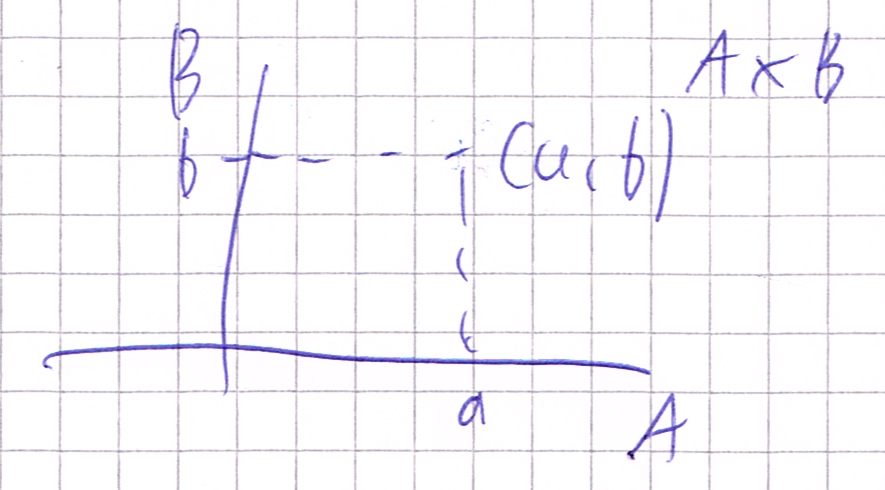
\includegraphics[width=0.3\textwidth]{img/1/3}
  \caption{Symbolische Zeichnung}
\end{figure}

\textbf{Zuweisung mit \qq{:=} bedeutet, das der Ausdruck auf Seite des Doppelpunkts durch die Gleichung definiert wird}.

Sei $X_1,\ldots,X_n$ Mengen, dann nennt man

\[\prod_{i=0}^n X_i := \{(x_1,\ldots,x_n):\text{für jedes } i \in \{1,\ldots,n\} \text{ ist } x_i \in X_i\}\]

Das \textbf{(kartesische) Produkt} der Mengen $X_1,\ldots,X_n$

$(x_1,\ldots,x_n)$ nennt man n-\textbf{Tupel}

$(x_1,\ldots,x_n)=(x_1',\ldots,x_n')$ gerade wenn $x_i=x_i'$ für jedes $\{1,\ldots,n\} $

Falls alle $x_i$ gleich einer Menge X sind, dann schreibt man

\[X^n = X \times \ldots \times X\] 

Die Begriffe Vereinigung und Durchschnitt erweitern sich auch auf mehr als zwei mengen:

\[\bigcap_{i=1}^n X_i = X_1 \cap \ldots \cap X_n := \{x : \text{für jedes }i \in \{1,\ldots,n\} \text{ gilt: } x \in X_i \}\]

\[\bigcup_{i=1}^n X_i = X_1 \cup \ldots \cup X_n := \{x : \text{es gibt ein }i \in \{1,\ldots,n\} \text{ mit } x \in X_i \}\]

\subsection{1.2 Logische Notationen}

Im folgenden steht A und B für (mathematische) Aussagen

Hier ein Beispiel:

$A=$ \qq{3 ist eine Primzahl}

$B=$ \qq{4 ist ungerade}

Hier ist A eine wahre und B eine falsche Aussage.

Man kann Aussagen wie folgt verknüpfen:

\begin{itemize}
  \item 1) Das \textbf{logische Und} von A und B - bezeichnet durch $A \wedge B$ - ist die Aussage \qq{A und B}
  \item 2) Das \textbf{logische Oder} von A und B - bezeichnet durch $A \vee B$ - ist die Aussage \qq{A oder B}
  \item 3) Die \textbf{Negation} von A - bezeichnet als $\lnot A$ - ist die Aussage \qq{nicht A}
\end{itemize}

Zusammengesetzte Verknüpfungen

\begin{itemize}
  \item Die \textbf{Implikation} von A nach B ist definiert als $(\lnot A) \vee B$ und wird mit $A \Longrightarrow B$ bezeichnet. Sie entspricht der Aussage \qq{wenn A, dann B}.
  \item Die \textbf{Äquivalenz} von A und B ist definiert als $(A \wedge B) \vee ((\lnot A)\wedge(\lnot B)) $ und wird mit $A \Longrightarrow B$ bezeichnet. Sie entspricht der Aussage \qq{A genau dann, wenn B}
\end{itemize}

Weiter verwendet man den \textbf{Allquantor} $\forall$ und den \textbf{Existenzquantor} $\exists$, die so zu lesen sind:

$\forall (1) : (2)$ \quad als: \quad Jedes (1) erfüllt (2)
$\exists (1) : (2)$ \quad als: \quad Es gilt ein (1), das (2) erfüllt

alternative Schreibweise: $\forall_{(1)} (2)$ und $\exists_{(1)} (2)$

\textbf{Beispiel} Die Aussage, dass $A \subseteq R$ nach oben beschränkt ist, lässt damit so formulieren:

$\exists s \in \mathbb{R} \forall a \in A: a < s$

\textbf{Beispiel} Sei $n \in \{1,3,4,\ldots\}$. Die Aussage, \qq{n ist prim} ist:

$ \forall \in \mathbb{N} \forall b \in \mathbb{N}:((a<n \wedge b < n) \Longrightarrow a*b \neq n)$

Es gilt offensichtlich: 

$\lnot \exists (1) : (2) \Longleftrightarrow \forall (1):\lnot (2)$

$\lnot \forall (1) : (2) \Longleftrightarrow \exists (1):\lnot (2)$

\textbf{ODER}

$\lnot \exists_{(1)} : (2) \text{ gdw. } \forall_{(1)}:\lnot (2)$

$\lnot \forall_{(1)} : (2) \text{ gdw. } \exists_{(1)}:\lnot (2)$

\textbf{Die Umkehrung für Oben lauter}

\subsection{Abbildungen}

\subsubsection{Definition 1.3}

Sei X und Y Mengen. Eine Abbildung $f:X \to Y$ (oder $f:X \stackrel{f}{\to}$) ist eine  
Vorschrift, die jedem $x \in X$ genau ein Element $f(x) \in Y$ zuordnet.

Dabei heißt $X$ \textbf{Definitionsbereich} und $Y$ \textbf{Wertebereich}.

\subsubsection{Definition 1.4}

Sei $f:X \to Y$ eine Abbildung und $A \subset X$ und $B \subset Y$. Dann heißt

\[f(A)=\{f(x)|x \in A\}\]

Das \textbf{Das Bild von A}

Weiter heißt \[f^{-1}(B)=\{x\in X|f(x) \in B\}\]

\textbf{Urbild} von B.

\textbf{Beispiele}

\begin{enumerate}
 \item $f: \mathbb{R} \to \mathbb{R}, x \mapsto x^2$
 \item $f: \mathbb{R} \to \{-1,1\} \mapsto \left\{ 
    \begin{array}{rl}
       -1, & \text{ falls } x \in \mathbb{Q} \\
        1, & \text{ falls } x \notin \mathbb{Q}
    \end{array}\right.$
 \item $f: \mathbb{R} \to \mathbb{R}, x \mapsto \frac{1}{x}$ ist \textbf{keine} gültige Abbildungsvorschrift!
 \item Seien $A,B$ Mengen. Dann nennt man $\pi_A \times B \to A, (a,b) \mapsto a$ \\
   eine \textbf{kanonische Projektion} auf $A$ \\
    \begin{figure}[h!]
      \centering
        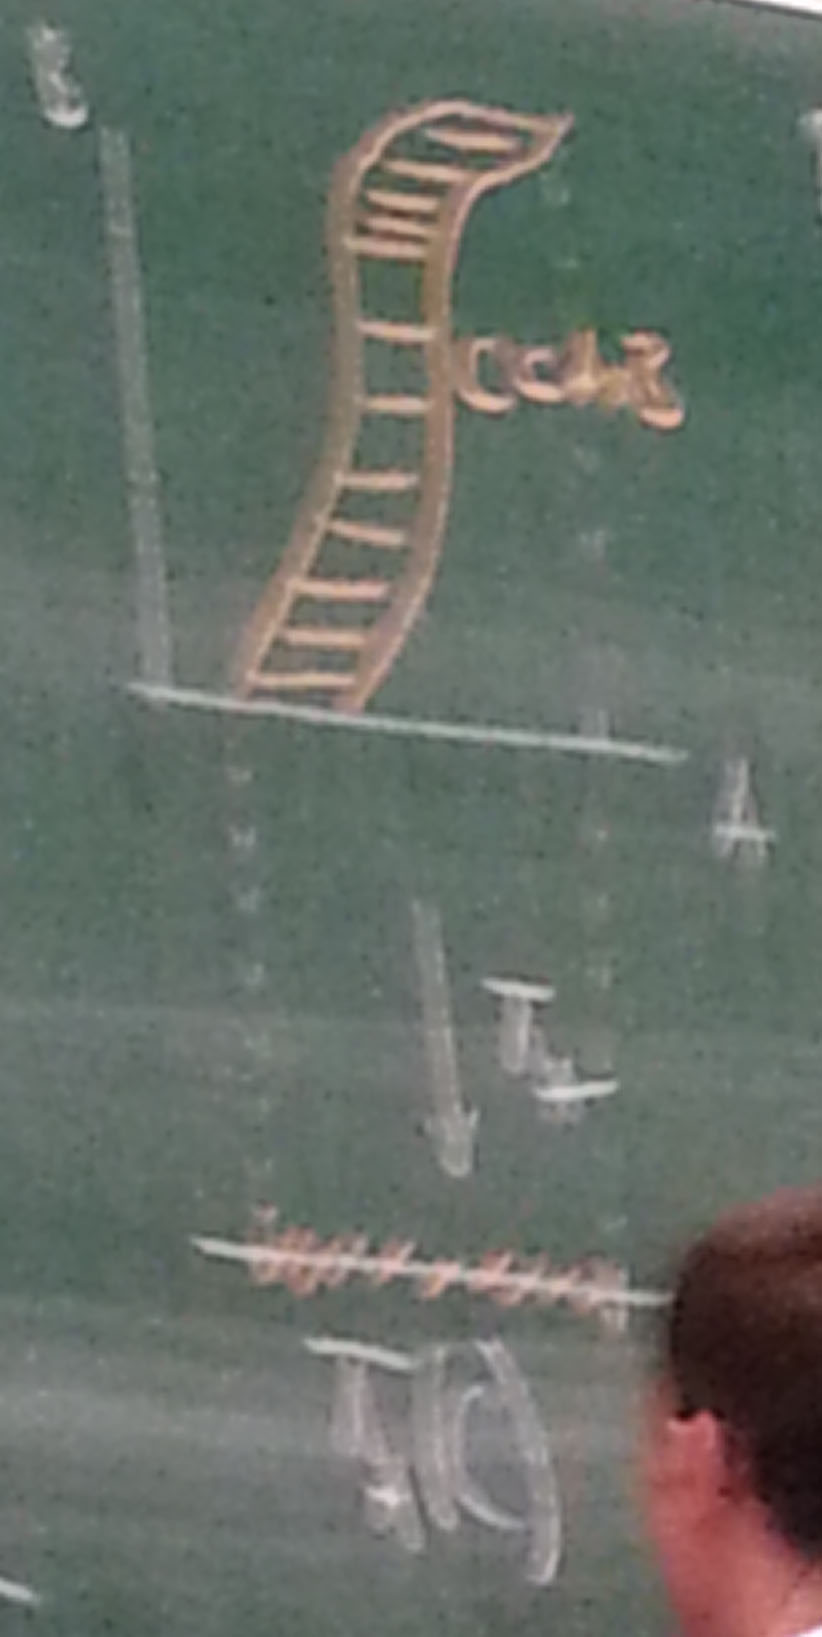
\includegraphics[width=100pt,height=200pt]{img/1/1}
        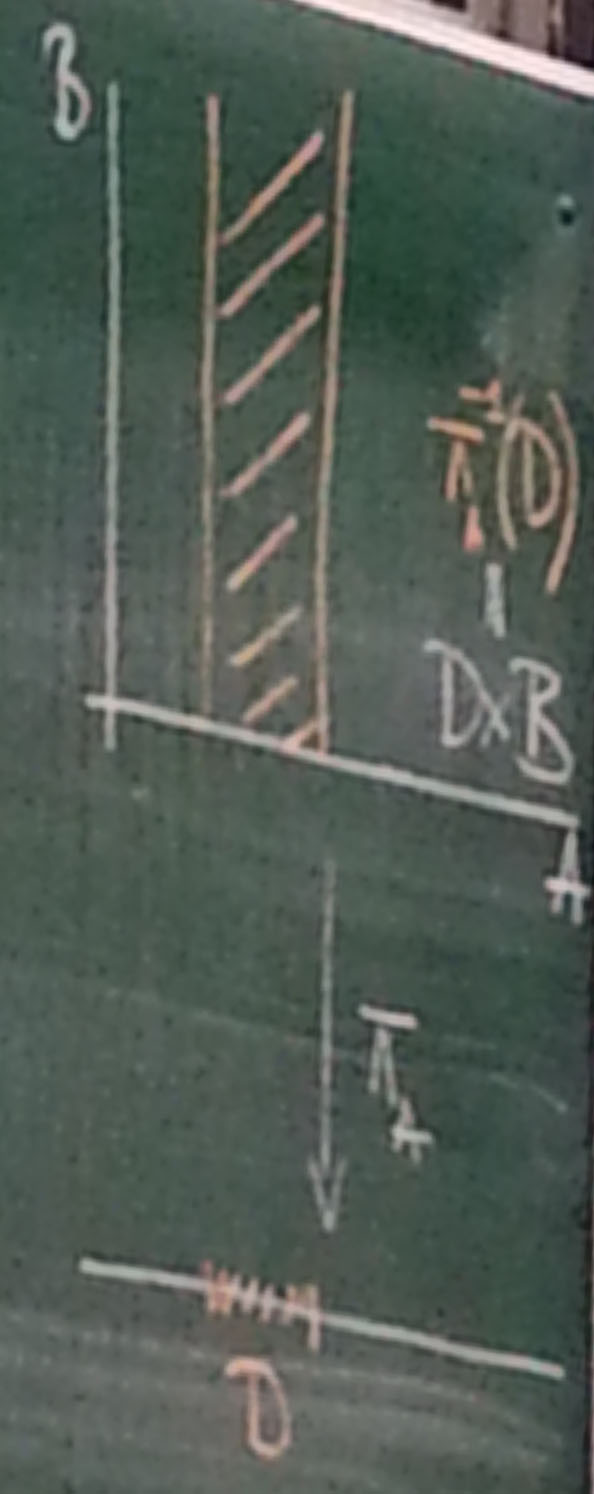
\includegraphics[width=100pt,height=200pt]{img/1/2}
      \caption{Zeichnung einer kanonische Projektion und seiner Umkehrabbildung}
    \end{figure} 
 \item Seien $A,B$ Mengen. Sei $b \in B$ Die Abbildung $f:A\to B, x \mapsto b$
\end{enumerate}

\subsubsection{Definition 1.6}

Seien $A$ eine Menge.

Die Abbildung

$id_A:A\to A, x \mapsto x$

heißt \textbf{Identität} auf $A$.

\subsubsection{Definition 1.7}

Sind $X \stackrel{f}{\to} Y$ und $Y \stackrel{g}{\to} Z$ Abbildungen, so ist die \textbf{Komposition} $g\circ f$ definiert als

$X \stackrel{g \circ f}{\to} Z,x \mapsto g(f(x))$

Mehrere Abbildungen kann man oft übersichtlich durch ein Diagramm darstellen, z.B.

\begin{displaymath}
    \xymatrix{
        A \ar[r]^f \ar[dr]_h & B \ar[d]^{g} \\
                            & C }
\end{displaymath}

\subsubsection{Definition 1.8}

Wenn in einem Diagramm zu je zwei Mengen alle Abbildungen \\
(auch (Mehrfach-)Kompositionen), die die eine Menge in die andere \\ 
Mengen abbilden, übereinstimmen, dann nennt man das Diagramm \textbf{Kommutativ}.

\begin{displaymath}
    \xymatrix{
        A \ar[r]^f \ar[d]_h & B \ar[d]^{g} \\
        C \ar[r]_{i}       & D }
\end{displaymath}

ist genau dann Kommutativ, wenn gilt:

$g \circ f = k \circ h$

\subsubsection{Definition 1.10}

Eine Abbildung $f:X \to Y$ heißt \textbf{injektiv}, wenn keine zwei Elemente in $X$ auf dasselbe Element in $Y$ abgebildet werden.

Sie heißt \textbf{surjektiv} wenn $f(X)=Y$ gilt.

Sie heißt \textbf{bijektiv}, wenn sie injektiv und surjektiv ist. 

\textbf{Beispiel}

\begin{enumerate}
  \item $f: \mathbb{R} \to \{x \in \mathbb{R}>0\}, f(x)=x^2$ \\
    ist nicht injektiv, z.B. $f(-1)=f(1)$ \\
    ist surjektiv (Beweis später)
  \item $\pi_A : A \times B \to A$ \\
    nicht injektiv, falls B mehr als ein Element besitzt $\pi_A((a,b))=\pi_A((a,b'))$ \\
    surjektiv, wenn $B \neq \emptyset$, wenn $b \in B$, dann ist $\pi_A((a,b))=a$ für jedes $a \ in A$ somit gilt $\pi_A(A \times B)=A$
\end{enumerate}

\subsubsection{Definition 1.11}

Sei $f: X \to Y$ eine bijektive Abbildung. Dann nennt man

$f^{-1}:Y \to X,f(x) \mapsto x$

die \textbf{Umkehrabbildung} von $f$.

\textbf{Wichtig:} $f(x) \to x$ ist nur dann eine gültige Abbildungsvorschrift, wenn $f$ bijektiv ist.    

\textbf{Bemerkung}

\begin{itemize}

\item Sei $X \stackrel{f}{\to}Y$ bijektiv.

Dann gilt $f^{-1} \circ f = id_X$ und

$f \circ f^{-1} = id_Y$ und

Denn $(f^{-1} \circ f )(x)=f^{-1}(f(x))=x=id_X(x)$

Sei $y \in Y$. Sei $x \in X$ mit $f(x)=y$

$(f \circ f^{-1})(y)=f(f^{-1}(y))=f(\underbrace{f^{-1}(f(x))}_{x})=f(x)=y=id_Y(y)$

\item Sei $f: X \to Y$ eine Abbildung

\textbf{Behauptung:} Wenn es eine Abbildung $g:Y \to X$ mit

$f \circ g = id_Y$ und

$g \circ f = id_X$,

dann ist $f$ bijektiv.

\textbf{Begründung} für "$f$ ist injektiv":

Seien $x,x' \in X$ mit $f(x)=f(x')$.

Somit $\underbrace{g(f(x))}_{x}=\underbrace{g(f(x'))}_{x}$ also $x=x'$

\textbf{Begründung} für "$f$ surjektiv": 

Sei $y \in Y$ Dann ist $f(g(y))=y$

\end{itemize}

\textbf{Beispiele}

\begin{enumerate}
  \item $f:\mathbb{R} \backslash \{0\} \to \mathbb{R} \backslash \{0\}, x\mapsto \frac{1}{x}$

ist bijektiv, es gilt $f^{-1}=f$

Denn: $f(f(x))=\frac{1}{\frac{1}{x}}=x=id_{f:\mathbb{R} \backslash \{0\}}$  
  
  \item $g:\mathbb{N} \to \mathbb{N}, n \mapsto n+1$ ist 
  
  
  \textbf{nicht} surjektiv, weil $1 \notin g(\mathbb{N})$.
  
  Dagegen ist $gg: \mathbb{Z} \to \mathbb{Z}, n \mapsto n+1$
  
  bijektiv mit $gg^{-1}(n)=n-1$ 
\end{enumerate}

\subsubsection{Definition 1.12}

\subsection{Äquivalenzrelationen}

Unter einer \textbf{Relation} auf einer Menge $X$ verstehen wir eine Teilmenge von $X \times X$.

Eine Teilmenge $R \subset X \times X$ so zu nennen, geht damit einher, die Aussage "$(x,y)\in R$" durch ein gewöhnliches "Relationssymbol" wie z.B. $\leq$ oder "$\thicksim$" als "$x \leq y$" oder "$x \thicksim y$" zu bezeichnen.

\subsubsection{Definition 1.12}

Eine Relation $\thicksim$ auf einer Menge $X$ heißt \textbf{Äquivalenzrelation}, \\
wenn sie \textbf{reflexiv}, \textbf{symmetrisch} und transitiv ist. d.h. wenn die Elemente von $X$ folgende Eigenschaften erfüllen:

\begin{enumerate}
 \item Für jedes $x \in X$ gilt $x \thicksim x$
 \item Aus $x \thicksim y$ folgt stets $y \thicksim x$
 \item Aus $x \thicksim y$ und $y \thicksim z$ folgt stets $x \thicksim z$
\end{enumerate}

Für jedes $x\in X$ heißt dann

\[[x]:= \{y \in X:y \thicksim x\} \subset X\]

Die \textbf{Äquivalenzklasse} von $x$.

Die Menge aller Äquivalenzklassen

$X/\thicksim := \{[x]:x \in X\}$

heißt \textbf{Quotientenmenge} von $X$ nach $\thicksim$. 

Die Abbildung 

$\begin{array}{rl}
    \pi: X \to & X/\thicksim \\
    x \mapsto  & [x]
\end{array}$

die jedem Element seine Äquivalenzklasse zuordnet, nennt man \textbf{Quotientenabbildung} oder auch \textbf{kanonische Projektion}.

\textbf{1.1.3: Kongruenzrelation}

Sein $n \in \mathbb{N}$. Sei $\equiv_n$ die Relation auf $\mathbb{Z}$, die durch 

\[x \equiv_n y :\Longleftrightarrow \exists k \in \mathbb{Z}: k*n=x-y\]

$: \Longleftrightarrow:$ Der Teil auf der Seite des Doppelpunkts wird dadurch definiert

Definiert wird.

\textbf{Beh:} $\equiv_n$ ist eine Äquivalenzrelation.

\textbf{Beweis:}

\begin{description}
  \item[Reflexivität:] $0*n=x-x \Longrightarrow x \equiv_n x$
  \item[Symmetrie:] Sei $x \equiv_n y$. Dann gibt es ein $k \in \mathbb{Z}$ mit $k*n=x-y$, somit $(-k)*n=y-x$. \\
  Also gilt $y=\equiv_n x$
  \item[Transitivität:] Seien $x\equiv_n y$ und $y \equiv_n z$. Somit gilt es $k,l \in \mathbb{Z}$ so dass $\left\{ 
    \begin{array}{l}
        k*n=xy \\
        l*n=y-x 
    \end{array}\right.$ 
    Daher $x-z=x-y
    y-z=(k+l)*n$ und somit $x \equiv_n z$
\end{description}

Äquivalenzklasse von $\equiv_n$:

Sei $x \in \mathbb{Z}$. Dann:
\[[x]=\{x+k*n:k\in \mathbb{Z}\}\]
Es gilt:
\[\mathbb{Z}/\equiv_n = {[0],[1],...,[n+1]}\]

\textbf{anschaulich:} Die zahlen $[i], 0\leq i \leq n-1$, sind genau die Zahlen, die bei Division mit $n$ Rest $i$ haben. 

Zwei Mengen $A$ und $B$ heißen \textbf{disjunkt}, wenn $A \cup B = \emptyset$. Eine Menge $M$ von Mengen heißt \textbf{paarweise disjunkt}, wenn zwei Mengen aus $M$ disjunkt sind.

Eine \textbf{Zerlegung} $\mathcal{Z}$ einer Menge $X$ ist eine paarweise disjunkte Menge von nicht-leeren Teilmengen von $X$.deren Vereinigung ganz $X$ ist  

Sei eine Zerlegung $\mathcal{Z}$ einer Menge $X$ gegeben.

Sei $\thicksim_{\mathcal{Z}}$ die Relation auf $X$, die durch

\[x \thicksim_{\mathcal{Z}} y : \Longleftrightarrow \exists Z \in \mathcal{Z}:\{x,y\}\subset Z,\]
definiert wird

\[\thicksim_{\mathcal{Z}}\] ist dann eine Äquivalenzrelation

\begin{description}
  \item[Reflexivität:] folgt $\bigcap Z = X$
  \item[Symmetrie:] ist offensichtlich.
  \item[Transitivität:] Sei $x \thicksim_{\mathcal{Z}} y$ und $y \thicksim_{\mathcal{Z}} z$. Dann gibt es $Z_1,Z_2 \in \mathcal{Z}$ mit $\{x,y\} \subset Z_1$ und $\{y,z\} \subset Z_2$. Da $\mathcal{Z}$ paarweise disjunkt ist, folgt $Z_1=Z_2$. Daher $\{x,z\}\subset Z_1$ also $x \thicksim_{\mathcal{Z}} z$
\end{description}

Es gilt also: $X/\thicksim_{\mathcal{Z}} = \mathcal{Z}$

\textbf{Satz 1.14:} Ist $\thicksim$ eine Äquivalenzrelation auf einer Menge $X$, dann ist die Menge der Äquivalenzklassen von $X$ eine Zerlegung von $X$ 

\textbf{Beweis}

Wegen Reflexivität ist $x\in[x]$.

Somit ist jede Äquivalenzklasse nicht leer.

Aus dem selben Grund enthält 

Z.z. bleibt: Zwei verschiedene Äquivalenzklassen sind disjunkt.

Sei $z \in [x] \cap [y]$ wir müssen $[x]=[y]$ zeigen.

Aus Symmetriegründen reicht es, $[x] \subset [y]$ zu zeigen.

Sei $u \in [x]$, also $u \thicksim x$

Wegen $z \in [x] \cap [y]$ ist $z \thicksim x$ und $z \thicksim y$

Wegen Symmetrie gilt auch $x \thicksim z$

Transitivität impliziert $u \thicksim Z$

Nochmals Transitivität impliziert $n\thicksim y$, also $u \in [y]$ 

\textbf{Beispiel} Betrachte die Äquivalenzrelation $\thicksim$ auf $\mathbb{R}^2$ definiert durch.

$(x,y) \thicksim (x',y') : \Longleftrightarrow y=y'$

Tatsächlich gibt es eine Bijektion:

$\begin{array}{rl}
    f: \mathbb{R} \to & \mathbb{R}^2/\thicksim \\
    x \mapsto & [(0,x)]
\end{array}$

Injektiv: $[(0,x)]=[(0,x')] \Longleftrightarrow x=x'$
 
Surjektiv: Sei $[(a,b)]\in \mathbb{R}^2/\thicksim$ Dann ist $[(a,b)] = [(0,b)]=f(b)$

$[x]=[y] \Longleftrightarrow x \thicksim y$

Falls \textbf{nicht} $x \thicksim y$, dann $[x] \cap [y]=\emptyset$

Ist $\thicksim$ eine Äquivalenzrelation auf $X$, so heißt $x \in X$ \textbf{Repräsentant} oder \textbf{Vertreter} von $[x]$

Nicht-Eindeutigkeit von Repräsentanten $\leadsto$ Problem der \textbf{Wohldefiniertheit}

\textbf{Bemerkung 1.15}: Ist $f:X \to Y$ eine Abbildung und $\thicksim$ eine Äquivalenzrelation auf $X$, so ist durch 
\[X/\thicksim \to Y, [x] \mapsto f(x)\]
eine Abbildung nur dann definiert, wenn 
\[x\thicksim x' \Longrightarrow f(x)=f(x')\]

gilt.

Anderenfalls sagt man: Die Abbildung ist nicht wohldefiniert. 

$\begin{array}{rl}
    g: \mathbb{R}^2/\thicksim & \to     \mathbb{R} \\
           \left[(a,b)\right] & \mapsto g([(a,b)]):=b
\end{array}$

\section{Algebraische Grundbegriffe}

\subsection{2.1 Gruppen}

Unter einer \textbf{Verknüpfung} auf einer Menge $M$ verstehen wir eine Abbildung 

$\begin{array}{rl}
    M \times M \to & M \\
    (m_1,m_2) \mapsto & m_1*m_2
\end{array}$

\textbf{Definition 2.1}

Verknüpfung $G \times G \to G, (g,h) \mapsto g*h$

heißt eine \textbf{Gruppe}, wenn folgendes gilt:

\begin{enumerate}
 \item (Assoziativität) \\
 	$\forall a,b,c \in G: (a*b)*c=a*(b*c)$
 \item (Neutrales Element) \\
    $\exists e \in G \forall a \in G: e*a=a*e=a$
 \item (Inverses) \\
    Zu jedem $a\in G$ gibt es ein sog. \textbf{Inverses}. d.h. ein Element $b \in G$ mit $a*b=b*a=e$ \\
    Das Inverse $e$  ist eindeutig (siehe 2) man schreibt dafür $a^{-1}$
\end{enumerate}

Weiter heißt $G$ \textbf{kommutativ} oder \textbf{abelsch}, wenn zusätzlich $a*b=b*a$ für alle $a,b \in G$ gilt.

\end{document}
